
\documentclass[letterpaper,hide notes,xcolor={table,svgnames},pdftex,10pt]{beamer}
\def\showexamples{t}


%\usepackage[svgnames]{xcolor}

%% Demo talk
%\documentclass[letterpaper,notes=show]{beamer}

\usecolortheme{crane}
\setbeamertemplate{navigation symbols}{}

\usetheme{MyPittsburgh}
%\usetheme{Frankfurt}

%\usepackage{tipa}

\usepackage{hyperref}
\usepackage{graphicx,xspace}
\usepackage[normalem]{ulem}
\usepackage{multicol}
\usepackage{amsmath,amssymb,amsthm,graphicx,xspace}
\newcommand\SF[1]{$\bigstar$\footnote{SF: #1}}

\usepackage[default]{sourcesanspro}
\usepackage[T1]{fontenc}
\usepackage[scaled]{beramono}
\usepackage{tikzpagenodes}

\newcounter{tmpnumSlide}
\newcounter{tmpnumNote}


% old question code
%\newcommand\question[1]{{$\bigstar$ \small \onlySlide{2}{#1}}}
% \newcommand\nquestion[1]{\ifdefined \presentationonly \textcircled{?} \fi \note{\par{\Large \textbf{?}} #1}}
% \newcommand\nanswer[1]{\note{\par{\Large \textbf{A}} #1}}


 \newcommand\mnote[1]{%
   \addtocounter{tmpnumSlide}{1}
   \ifdefined\showcues {~\tiny\fbox{\arabic{tmpnumSlide}}}\fi
   \note{\setlength{\parskip}{1ex}\addtocounter{tmpnumNote}{1}\textbf{\Large \arabic{tmpnumNote}:} {#1\par}}}

\newcommand\mmnote[1]{\note{\setlength{\parskip}{1ex}#1\par}}

%\newcommand\mnote[2][]{\ifdefined\handoutwithnotes {~\tiny\fbox{#1}}\fi
% \note{\setlength{\parskip}{1ex}\textbf{\Large #1:} #2\par}}

%\newcommand\mnote[2][]{{\tiny\fbox{#1}} \note{\setlength{\parskip}{1ex}\textbf{\Large #1:} #2\par}}

\newcommand\mquestion[2]{{~\color{red}\fbox{?}}\note{\setlength{\parskip}{1ex}\par{\Large \textbf{?}} #1} \note{\setlength{\parskip}{1ex}\par{\Large \textbf{A}} #2\par}\ifdefined \presentationonly \pause \fi}

\newcommand\blackboard[1]{%
\ifdefined   \showblackboard
  {#1}
  \else {\begin{center} \fbox{\colorbox{blue!30}{%
         \begin{minipage}{.95\linewidth}%
           \hspace{\stretch{1}} Some space intentionally left blank; done at the blackboard.%
         \end{minipage}}}\end{center}}%
         \fi%
}



%\newcommand\q{\tikz \node[thick,color=black,shape=circle]{?};}
%\newcommand\q{\ifdefined \presentationonly \textcircled{?} \fi}

\usepackage{listings}
\lstset{basicstyle=\footnotesize\ttfamily,
	breaklines=true,
	aboveskip=15pt,
  	belowskip=15pt,
	frame=lines,
	numbers=left, basicstyle=\scriptsize, numberstyle=\tiny, stepnumber=0, numbersep=2pt
}

\usepackage{siunitx}
\newcommand\sius[1]{\num[group-separator = {,}]{#1}\si{\micro\second}}
\newcommand\sims[1]{\num[group-separator = {,}]{#1}\si{\milli\second}}
\newcommand\sins[1]{\num[group-separator = {,}]{#1}\si{\nano\second}}
\sisetup{group-separator = {,}, group-digits = true}

%% -------------------- tikz --------------------
\usepackage{tikz}
\usetikzlibrary{positioning}
\usetikzlibrary{arrows,backgrounds,automata,decorations.shapes,decorations.pathmorphing,decorations.markings,decorations.text,decorations.pathreplacing}

\tikzstyle{place}=[circle,draw=blue!50,fill=blue!20,thick, inner sep=0pt,minimum size=6mm]
\tikzstyle{transition}=[rectangle,draw=black!50,fill=black!20,thick, inner sep=0pt,minimum size=4mm]

\tikzstyle{block}=[rectangle,draw=black, thick, inner sep=5pt]
\tikzstyle{bullet}=[circle,draw=black, fill=black, thin, inner sep=2pt]

\tikzstyle{pre}=[<-,shorten <=1pt,>=stealth',semithick]
\tikzstyle{post}=[->,shorten >=1pt,>=stealth',semithick]
\tikzstyle{bi}=[<->,shorten >=1pt,shorten <=1pt, >=stealth',semithick]

\tikzstyle{mut}=[-,>=stealth',semithick]

\tikzstyle{treereset}=[dashed,->, shorten >=1pt,>=stealth',thin]

\usepackage{ifmtarg}
\usepackage{xifthen}
\makeatletter
% new counter to now which frame it is within the sequence
\newcounter{multiframecounter}
% initialize buffer for previously used frame title
\gdef\lastframetitle{\textit{undefined}}
% new environment for a multi-frame
\newenvironment{multiframe}[1][]{%
\ifthenelse{\isempty{#1}}{%
% if no frame title was set via optional parameter,
% only increase sequence counter by 1
\addtocounter{multiframecounter}{1}%
}{%
% new frame title has been provided, thus
% reset sequence counter to 1 and buffer frame title for later use
\setcounter{multiframecounter}{1}%
\gdef\lastframetitle{#1}%
}%
% start conventional frame environment and
% automatically set frame title followed by sequence counter
\begin{frame}%
\frametitle{\lastframetitle~{\normalfont(\arabic{multiframecounter})}}%
}{%
\end{frame}%
}
\makeatother

\makeatletter
\newdimen\tu@tmpa%
\newdimen\ydiffl%
\newdimen\xdiffl%
\newcommand\ydiff[2]{%
    \coordinate (tmpnamea) at (#1);%
    \coordinate (tmpnameb) at (#2);%
    \pgfextracty{\tu@tmpa}{\pgfpointanchor{tmpnamea}{center}}%
    \pgfextracty{\ydiffl}{\pgfpointanchor{tmpnameb}{center}}%
    \advance\ydiffl by -\tu@tmpa%
}
\newcommand\xdiff[2]{%
    \coordinate (tmpnamea) at (#1);%
    \coordinate (tmpnameb) at (#2);%
    \pgfextractx{\tu@tmpa}{\pgfpointanchor{tmpnamea}{center}}%
    \pgfextractx{\xdiffl}{\pgfpointanchor{tmpnameb}{center}}%
    \advance\xdiffl by -\tu@tmpa%
}
\makeatother
\newcommand{\copyrightbox}[3][r]{%
\begin{tikzpicture}%
\node[inner sep=0pt,minimum size=2em](ciimage){#2};
\usefont{OT1}{phv}{n}{n}\fontsize{4}{4}\selectfont
\ydiff{ciimage.south}{ciimage.north}
\xdiff{ciimage.west}{ciimage.east}
\ifthenelse{\equal{#1}{r}}{%
\node[inner sep=0pt,right=1ex of ciimage.south east,anchor=north west,rotate=90]%
{\raggedleft\color{black!50}\parbox{\the\ydiffl}{\raggedright{}#3}};%
}{%
\ifthenelse{\equal{#1}{l}}{%
\node[inner sep=0pt,right=1ex of ciimage.south west,anchor=south west,rotate=90]%
{\raggedleft\color{black!50}\parbox{\the\ydiffl}{\raggedright{}#3}};%
}{%
\node[inner sep=0pt,below=1ex of ciimage.south west,anchor=north west]%
{\raggedleft\color{black!50}\parbox{\the\xdiffl}{\raggedright{}#3}};%
}
}
\end{tikzpicture}
}


%% --------------------

%\usepackage[excludeor]{everyhook}
%\PushPreHook{par}{\setbox0=\lastbox\llap{MUH}}\box0}

%\vspace*{\stretch{1}

%\setbox0=\lastbox \llap{\textbullet\enskip}\box0}

\setlength{\parskip}{\fill}

\newcommand\noskips{\setlength{\parskip}{1ex}}
\newcommand\doskips{\setlength{\parskip}{\fill}}

\newcommand\xx{\par\vspace*{\stretch{1}}\par}
\newcommand\xxs{\par\vspace*{2ex}\par}
\newcommand\tuple[1]{\langle #1 \rangle}
\newcommand\code[1]{{\sf \footnotesize #1}}
\newcommand\ex[1]{\uline{Example:} \ifdefined \presentationonly \pause \fi
  \ifdefined\showexamples#1\xspace\else{\uline{\hspace*{2cm}}}\fi}

\newcommand\ceil[1]{\lceil #1 \rceil}


\AtBeginSection[]
{
   \begin{frame}
       \frametitle{Outline}
       \tableofcontents[currentsection]
   \end{frame}
}



\pgfdeclarelayer{edgelayer}
\pgfdeclarelayer{nodelayer}
\pgfsetlayers{edgelayer,nodelayer,main}

\tikzstyle{none}=[inner sep=0pt]
\tikzstyle{rn}=[circle,fill=Red,draw=Black,line width=0.8 pt]
\tikzstyle{gn}=[circle,fill=Lime,draw=Black,line width=0.8 pt]
\tikzstyle{yn}=[circle,fill=Yellow,draw=Black,line width=0.8 pt]
\tikzstyle{empty}=[circle,fill=White,draw=Black]
\tikzstyle{bw} = [rectangle, draw, fill=blue!20, 
    text width=4em, text centered, rounded corners, minimum height=2em]
    
    \newcommand{\CcNote}[1]{% longname
	This work is licensed under the \textit{Creative Commons #1 3.0 License}.%
}
\newcommand{\CcImageBy}[1]{%
	\includegraphics[scale=#1]{creative_commons/cc_by_30.pdf}%
}
\newcommand{\CcImageSa}[1]{%
	\includegraphics[scale=#1]{creative_commons/cc_sa_30.pdf}%
}
\newcommand{\CcImageNc}[1]{%
	\includegraphics[scale=#1]{creative_commons/cc_nc_30.pdf}%
}
\newcommand{\CcGroupBySa}[2]{% zoom, gap
	\CcImageBy{#1}\hspace*{#2}\CcImageNc{#1}\hspace*{#2}\CcImageSa{#1}%
}
\newcommand{\CcLongnameByNcSa}{Attribution-NonCommercial-ShareAlike}

\newenvironment{changemargin}[1]{% 
  \begin{list}{}{% 
    \setlength{\topsep}{0pt}% 
    \setlength{\leftmargin}{#1}% 
    \setlength{\rightmargin}{1em}
    \setlength{\listparindent}{\parindent}% 
    \setlength{\itemindent}{\parindent}% 
    \setlength{\parsep}{\parskip}% 
  }% 
  \item[]}{\end{list}} 




\title{Lecture 32 --- Convergence, Ergodicity, Applications}

\author{Jeff Zarnett\\ \small \texttt{jzarnett@uwaterloo.ca}}
\institute{Department of Electrical and Computer Engineering \\
  University of Waterloo}
\date{\today}


\begin{document}

\begin{frame}
  \titlepage

 \end{frame}


\begin{frame}
\frametitle{Convergence}

An image of what convergence looks like:

\begin{center}
	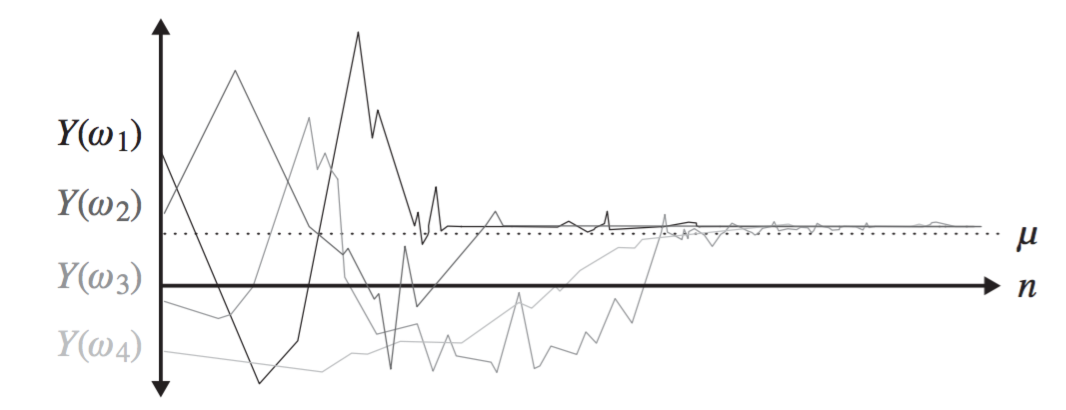
\includegraphics[width=0.6\textwidth]{images/convergence.png}
\end{center}

We won't concern ourselves with systems where there is no convergence. 

\end{frame}



\begin{frame}
\frametitle{Tim and Enzo}

A small but important digression on the subject of sampling, measurement, and testing.

You have an idea of what an average is, but there are two different types of average---the time average and ensemble average. 


\end{frame}



\begin{frame}
\frametitle{Tim and Enzo Scenario}

Let us just focus on having a single First-Come-First-Serve queue. 

Every second, a new job arrives with probability $p$ and if there is any work to do, the job being worked on is completed with probability $q$ (and $q > p$). 

As a definition, let $N(v)$ equal the number of jobs in the system at a time $v$. 

In the story, Tim and Enzo are trying to simulate the FCFS system to determine what is the average number of jobs in the system.

\end{frame}



\begin{frame}
\frametitle{The Tim Approach}

Tim decides he's going to run it as one really long simulation. 

He simulates the queue over a very long period, logging as he goes, taking a million samples. 

Then he takes the average value over those samples to get the average number of jobs.

\end{frame}



\begin{frame}
\frametitle{The Enzo Approach}

Enzo does something slightly different: instead of having one super long simulation, he does 1000 shorter simulations. 

He waits until the simulation has run for 1000 seconds and then samples the queue at exactly that point, obtaining one value. 

This experiment is restarted with a new random seed. 

So after obtaining a thousand samples, he averages these, and Enzo produces another average number of jobs.


\end{frame}



\begin{frame}
\frametitle{Tim and Enzo}

\begin{center}
	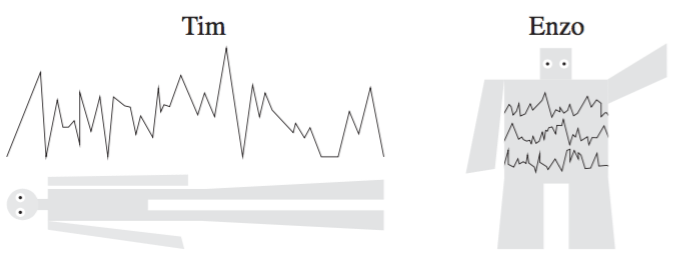
\includegraphics[width=0.8\textwidth]{images/timenzo.png}
\end{center}

So---who has done this correctly, Tim or Enzo?

\end{frame}



\begin{frame}
\frametitle{Time Average vs Ensemble Average}

The time average has potential problems because we are only looking at a single sequence and maybe something very unusual has happened here in this single run. 

The ensemble average is more likely what we talk about when we talk about the system being at ``steady state'' (i.e., past the initial conditions). 

So we kind of like the Enzo approach. Tim's approach still has some merit though.

\end{frame}



\begin{frame}
\frametitle{Initial Conditions}

Both the Tim and Enzo approaches here require caring about the initial conditions. 

Enzo needs to make sure that the initial conditions (startup costs etc) have attenuated before the measurement point. 

Tim needs to ensure that the initial conditions impact a sufficiently small portion of all his measurements.

\end{frame}



\begin{frame}
\frametitle{Everyone's a Winner}

If we have a nicely behaved system, the time average and the ensemble average are the same (so both Tim and Enzo can be correct). 

What is a nicely behaved system? The word for this is \alert{ergodic}. 

That probably did not help, so what is an ergodic system? 

It is a system that is positive recurrent, aperiodic, and irreducible.

\end{frame}



\begin{frame}
\frametitle{Irreducibility}

\alert{Irreducibility} means a process should be able to get from one state to any other state (where state is the number of jobs in the system). 

This means the initial state of the system does not matter. 

So if we started at 0 jobs or 10 we could still get to any state in the system (jobs at 2 or 27)...

\end{frame}



\begin{frame}
\frametitle{Positive Recurrence}

\alert{Positive recurrence} means that given an irreducible system, any state $i$ is revisited infinitely often, and the time between visits to that state are finite. 

So we can define a certain state as being a ``restart''. 

The logical choice in the case of a queue or similar is the idea of the queue being empty. 

Every time the queue gets down to zero jobs, it's a ``restart'' of sorts. 

\end{frame}



\begin{frame}
\frametitle{Positive Recurrence}

This is what makes Tim's view and Enzo's view potentially the same. 

A single long run (Tim's view) is just like a number of independent runs (Enzo's view). 

Every time we get down to zero jobs in the queue, it's a restart. 

\end{frame}



\begin{frame}
\frametitle{Aperiodicity}

The \alert{aperiodicity} condition is required for the ensemble average to make sense or exist. 

That is to say, the state of the system should not be related to the the time.

Otherwise the way Enzo chooses to sample, i.e., $t = 1000$, is potentially going to skew the result.

\end{frame}



\begin{frame}
\frametitle{Tim as Enzo}

\begin{center}
	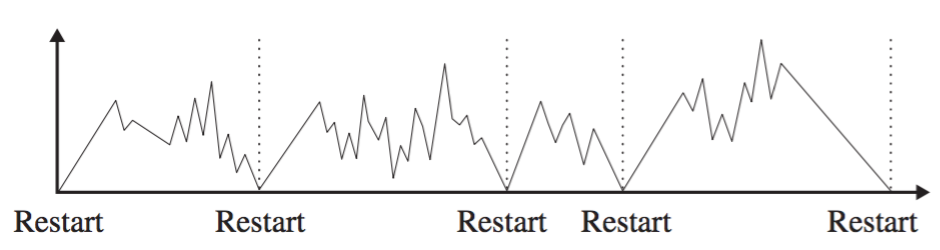
\includegraphics[width=0.8\textwidth]{images/systemrestart.png}
\end{center}

So both Tim and Enzo are correct, given an ergodic system.


\end{frame}



\begin{frame}
\frametitle{How Long Jobs Are in the System}

We could compute either the time or ensemble average. 

\begin{center}
	Time Average = $\lim_{t\to\infty}\dfrac{\sum_{i=1}^{A(t)} T_{i}}{A(t)}$
\end{center}

where $A(t)$ is the number of arrivals by time $t$ and $T_{i}$ is the time in the system of arrival $i$. The average is taken over one sample path.


\end{frame}

\begin{frame}
\frametitle{How Long Jobs Are in the System}

\begin{center}
	Ensemble Average = $\lim_{t\to\infty}E[T_{i}]$
\end{center}

where $E[T_{i}]$ is the average time in the system of job $i$, where the average is taken over all sample paths.


\end{frame}

\begin{frame}
\frametitle{Little's Law}

Little's Law says the average number of jobs in the system equals the product the average arrival rate into the system and the average time in the system. 

Let's start with an open system. The law, written more formally:

\begin{center}
	$E[N] = \lambda E[T]$
\end{center}

\end{frame}



\begin{frame}
\frametitle{Little's Law}

\begin{center}
	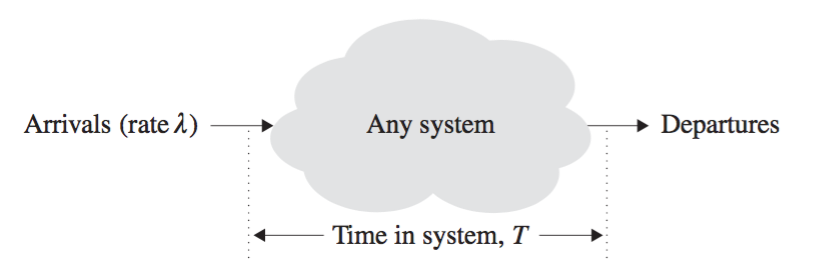
\includegraphics[width=0.8\textwidth]{images/littleslaw.png}
\end{center}

\end{frame}



\begin{frame}
\frametitle{Ignorance is Bliss}

\large
\begin{changemargin}{1.5cm}
What we don't need to know about:
\begin{itemize}
\item the arrival process;
\item the service time distribution;
\item network topology;
\item etc. 
\end{itemize}

It seems intuitive that this is the case (or it should be). 
\end{changemargin}

\end{frame}



\begin{frame}
\frametitle{Restaurant Analogy}

\begin{minipage}{.49\textwidth}
\begin{center}

\includegraphics[width=10em]{images/McDonalds-Logo-500x319.png}
\end{center}

Key: Quick turnaround time. \\

Get people out quickly (low $E[T]$) 

$\Rightarrow$ don't need a lot of seating (low $E[N]$)
\end{minipage} \begin{minipage}{.49\textwidth}
\begin{center}

\includegraphics[width=10em]{images/proof-logo.png}
\end{center}

\begin{changemargin}{1em}
Opposite situation: \\

people leave slowly (high $E[T]$) 

$\Rightarrow$ need much seating (more $E[N]$). 
\end{changemargin}
\end{minipage}

\end{frame}



\begin{frame}
\frametitle{FCFS Version}

\large
\begin{changemargin}{2cm}
Single FCFS queue:

\begin{center}
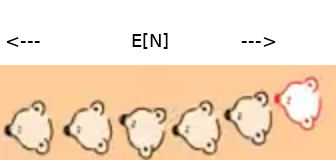
\includegraphics[width=15em]{images/L33-queue.png}
\end{center}

Expected time for each customer to complete: $1/\lambda$\\
\qquad because the average rate of completions is $\lambda $. 

So we can approximate $E[T]$ as roughly $\dfrac{1}{\lambda}E[N]$.
\end{changemargin}

\end{frame}



\begin{frame}
\frametitle{Little's Law for Closed Systems}

\large
\begin{changemargin}{2cm}

For closed systems:\\
\begin{itemize} 
\item $N$ jobs in process at any given time\\
\qquad (multiprocessing level of the system);
\item $X$ throughput rate.
\end{itemize}

If the system is ergodic, then $N = X \cdot E[T]$.

Assumes that there is zero think time.
 \end{changemargin}
\end{frame}



\begin{frame}
\frametitle{Users Ruin Everything}

\large
\begin{changemargin}{2cm}
If we do have to deal with users and think time, \\
then we care more about the response time $E[R]$. 

So for a terminal-driven system,\\
 expected response time is 
\end{changemargin}
~\\[-4em]
\[ E[R] = \dfrac{N}{X} - E[Z]. \]

\end{frame}



\begin{frame}
\frametitle{M/M/1}

\Large
\begin{changemargin}{2cm}
Probabilistic processes are described according to their models, which will probably be one of:

\begin{enumerate}
	\item Deterministic (D)	
	\item Markov (M)
	\item General (G)
\end{enumerate}
\end{changemargin}

\end{frame}



\begin{frame}
\frametitle{Markov Processes}

\large
\begin{changemargin}{1.5cm}
We'll focus on Markov processes. 
~\\[0em]
\begin{itemize}
\item Number of arrivals follows Poisson distribution.

\item Inter-arrival times follow exponential distribution. 

\item Service times follow exponential distribution.
\end{itemize}
\end{changemargin}

\end{frame}



\begin{frame}
\frametitle{Kendall Notation}

\Large
\begin{changemargin}{1.5cm}
Those letters we saw (D, M, G) are part of Kendall notation:

Six symbols, written in a specific order, separated by slashes. 

The order is $\alpha / \sigma / m / \beta / N / Q$. 
\end{changemargin}

\end{frame}



\begin{frame}
\frametitle{Kendall Notation}

\begin{center}
\begin{tabular}{ll} 
	\textbf{Symbol} & \textbf{Meaning} \\ \hline
	$\alpha$ & The type of distribution (Markov, General, Deterministic) \\ 
	$\sigma$ & The type of probability distribution for service time \\ 
	$m$ & Number of servers \\ 
	$\beta$ & Buffer size \\ 
	$N$ & Allowed population size (finite or infinite) \\ 
	$Q$ & Queueing policy \\ 
\end{tabular}
\end{center}

\end{frame}



\begin{frame}
\frametitle{Why is abbreviation such a long word?}

\large
\begin{changemargin}{1.5cm}
We often leave off the last three\\
assuming that there is an infinite buffer, infinite population, and a FIFO queueing policy. \\[1em]

If that is the case, then we have only three values. \\[1em]

This produces the ``M/M/1'' and ``M/M/k'' symbols. \\[1em]

``M/M/1'' means a Markov arrival process, exponential queueing system, and a single server. \\

\begin{itemize}
\item When there are $k$ servers, use $k$ instead of $1$.
\end{itemize}
\end{changemargin}

\end{frame}



\begin{frame}
\frametitle{Utilization}

\begin{center}
	
\includegraphics[width=0.4\textwidth]{images/weekend.png}
\end{center}

\large
\begin{changemargin}{1.5cm}
\[ \rho \text{ = utilization} \in [0, 1]\]
the amount of time that the server is busy. 

We talked about this earlier in an informal way, but now we can actually calculate it! \\[-1em]

\[ \rho = \lambda \times s.\]
\end{changemargin}

\end{frame}



\begin{frame}
\frametitle{M/M/1 Formul\ae}

\large
\begin{changemargin}{1.5cm}
For M/M/1 systems: \\[0em]

\begin{itemize}
\item completion time average, $T_{q}$, is $\dfrac{s\rho}{(1-\rho)}$
\item average length of queue, $W$, is $\dfrac{\rho^{2}}{1-\rho}$
\end{itemize}
\end{changemargin}
\end{frame}



\begin{frame}
\frametitle{Queuing Theory Example}

\large
\begin{changemargin}{1.5cm}
Server completes a request, on average, in 10~ms. 

Time to complete request is exponentially distributed. 

Over 30 minutes, 117~000 jobs arrive. 

$\Longrightarrow$ a M/M/1 situation. 

\begin{itemize}
\item How long did it take to complete the average request? 

\item What is the average queue length?
\end{itemize}
\end{changemargin}

\end{frame}



\begin{frame}
\frametitle{Queueing Theory Example}

\large
\begin{changemargin}{1.5cm}
Given: service time $s$ is $0.01s$, \\
arrival rate is 65 requests per second. 

We calculate $\rho = 0.01 \times 65 = 0.65$. 

Using the above formul\ae:

\begin{itemize}
\item Time to complete the average request is 28.6~ms. 

\item Average length of the queue is 1.21.
\end{itemize}
\end{changemargin}
\end{frame}



\begin{frame}
\frametitle{Queueing Theory Example}

\large
\begin{changemargin}{1.5cm}
What about the number of jobs in the system? 

$Q = \dfrac{\rho}{1-\rho}$ average number of jobs, \\
including the waiting jobs and the ones being served.  

The probability that there are\\
 exactly $x$ jobs in the system at any time is: 
\[ (1-\rho)\rho^{x}.\]
\end{changemargin}

\end{frame}



\begin{frame}
\frametitle{Queueing Theory Example}

\large
\begin{changemargin}{1.5cm}
The probability that the number of jobs\\
 is less than or equal to $n$ is: 

\[ \sum\limits_{i=0}^{n}(1-\rho)\rho^{i}. \]

For more than $n$ at a time, from $n+1$ to infinity\ldots Or \ldots

\[ 1 - \sum\limits_{i=0}^{n}(1-\rho)\rho^{i}. \]
\end{changemargin}

\end{frame}



\begin{frame}
\frametitle{M/M/k}

\large
\begin{changemargin}{1.5cm}
Next: multiple servers.

Jobs arrive at a single queue. \\
When a server is ready, \\
it takes the 1st job from front of queue. 

Servers are identical, jobs can be served by any server. 

So far, so simple. Sadly, the math just got harder. 
\end{changemargin}

\end{frame}




\begin{frame}
\frametitle{M/M/k}

\large
\begin{changemargin}{1.5cm}
The server utilization for the server farm is now 
\[ \rho = \lambda s / N. \]

To make our calculations a little easier, we want an intermediate value $K$:
\[ K = \cfrac{\sum_{i=0}^{N-1}\dfrac{(\lambda s)^{i}}{i!}}{{\sum_{i=0}^{N}\dfrac{(\lambda s)^{i}}{i!}}}.\]

$K$ is always less than 1. It has no intrinsic meaning.
\end{changemargin}

\end{frame}

\begin{frame}
\frametitle{M/M/k}

\large
\begin{changemargin}{1.5cm}
What is the probability that all servers are busy? 

$C = $ probability a new job will have to wait in queue.

\[
	C = \cfrac{1 - K}{1 - \dfrac{\lambda s K}{N}}.\]

The M/M/k formul\ae: \\[0em]

\[ T_{q} = \dfrac{C s}{k(1 - \rho)} + s \mbox{\qquad\qquad\qquad} W = C \dfrac{\rho}{1 - \rho} \]
\end{changemargin}

\end{frame}


\begin{frame}
\frametitle{Printer Example}

\large
\begin{changemargin}{1.5cm}
Our printer completes an average print job in 2 min. 

Every 2.5 minutes, a user submits a job to the printer. 

\begin{itemize}
\item How long does it take to get the print job on average? 
\end{itemize}

For a single printer, the system is M/M/1. 

Service time $s$ is 2 minutes; \\
arrival rate $\lambda$ is $1/2.5 = 0.4$. 

\begin{itemize}
\item $\rho = \lambda \times s = 0.4 \times 2 = 0.8$. 
\item $T_{q} = s\rho / (1 - \rho ) = 2 / (1 -0.8 ) = 8$. 
\end{itemize}

Eight minutes to get the print job. Ouch.
\end{changemargin}

\end{frame}

\begin{frame}
\frametitle{Printer Example}

\begin{center}
	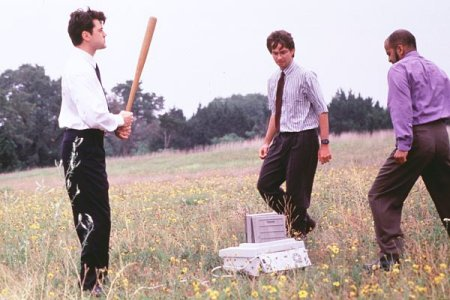
\includegraphics[width=0.5\textwidth]{images/printer.jpg}
\end{center}


\end{frame}

\begin{frame}
\frametitle{Executive Decision}

\large
\begin{changemargin}{1.5cm}
Here we have an opportunity to use the predictive power of queueing theory. 

Management is convinced that eight minute waits for print jobs is unreasonable, so we have been asked to decide what to do. 

\begin{itemize}
\item Should we buy a second printer of the same speed?
\item Or should we sell the old one and buy a printer that is double the speed?
\end{itemize}
\end{changemargin}

\end{frame}



\begin{frame}
\frametitle{New Printer}

\large
\begin{changemargin}{1.5cm}
The faster printer calculation is easy enough. 

Now $s = 1.0$ and $\lambda$ remains $0.4$, making $\rho = 0.4$. 

So rerunning the calculation: 
\[ T_{q} = s\rho / (1 - \rho ) = 1 / (1 - 0.4 ) = 0.67.\]
~\\[0em]

A lot less time!
\end{changemargin}

\end{frame}



\begin{frame}
\frametitle{Two Printer Solution}

\large
\begin{changemargin}{1.5cm}
The two printer solution is more complicated. \\
So let us calculate intermediate value $K$.

	\[ K = \cfrac{\sum_{i=0}^{N-1}\dfrac{(\lambda s)^{i}}{i!}}{{\sum_{i=0}^{N}\dfrac{(\lambda s)^{i}}{i!}}} = \cfrac{\dfrac{(\lambda s)^{0}}{0!} + \dfrac{(\lambda s)^{1}}{1!}}{\dfrac{(\lambda s)^{0}}{0!} + \dfrac{(\lambda s)^{1}}{1!} + \dfrac{(\lambda s)^{2}}{2!}} = 0.849057.
\]
	
\end{changemargin}
\end{frame}



\begin{frame}
\frametitle{Calculate!}

\large
\begin{changemargin}{1.5cm}
Now $C$ is 0.22857 and $T_{q}$ is 2.38 minutes. 

Two observations jump out at us: \\[0em]
\begin{enumerate}
\item we doubled the number of printers, but now jobs are completed almost four times faster; and 
\item the single fast printer is better, if utilization is low.
\end{enumerate}
\end{changemargin}
\end{frame}



\begin{frame}
\frametitle{Conditions}

\large
\begin{changemargin}{1.5cm}
That is an important condition: if utilization is low. 

At some point will the two printers be a better choice than the single fast one? 

What if both printers are used to the max (100\% load)...?
\end{changemargin}

\end{frame}



\begin{frame}
\frametitle{Queueing for Performance}

\large
\begin{changemargin}{1.5cm}
The basic process is:

\begin{enumerate}
	\item Convert to common time units.
	\item Calculate the visitation ratios $V_{i}$.
	\item Calculate the device utilization $\rho_{i}$.
	\item Calculate the CPU service time.
	\item Calculate the device time.
	\item Find the bottleneck device.
	\item Calculate the maximum transaction rate.
	\item Calculate the average transaction time.
\end{enumerate}
\end{changemargin}
\end{frame}



\begin{frame}
\frametitle{Queueing for Performance}

\begin{changemargin}{1cm}
\large Let us execute this process on a web server system that serves 9~000 pages per hour. Here are the known values:
\end{changemargin}

\begin{center}
\begin{tabular}{l|r|r|r|r|r|r} 
	\textbf{Device} & \textbf{Data/Hour} & \textbf{$\lambda$} & \textbf{$S$} & \textbf{$V$} & \textbf{$\rho$} & \textbf{$V \times S$} \\ \hline
	Webpages & 9~000 & & & & & \\ \hline
	CPU & & & & &  42\% & \\ \hline
	Disk 1 & 108~000 & & 11ms & & &\\ \hline
	Disk 2 & 72~000 & & 16ms & & &\\ \hline
	Network & 18~000 & & 23ms & & &\\ 
\end{tabular}
\end{center}

\end{frame}



\begin{frame}
\frametitle{Queueing for Performance}

\begin{changemargin}{1cm}
\large 
Step one is to convert to common time units; in this case, seconds.

Let's also look at the $\lambda$ values---reported counts divided by seconds in the reporting period.
\end{changemargin}

\begin{center}
\begin{tabular}{l|r|r|r|r|r|r} 
	\textbf{Device} & \textbf{Data/Hour} & \textbf{$\lambda$} & \textbf{$S$} & \textbf{$V$} & \textbf{$\rho$} & \textbf{$V \times S$} \\ \hline
	Webpages & 9~000 & 2.5 & & & & \\ \hline
	CPU & & & & & 42\% & \\ \hline
	Disk 1 & 108~000 & 30 & 0.011s  & & &\\ \hline
	Disk 2 & 72~000 & 20 & 0.016s & & &\\ \hline
	Network & 18~000 & 5 & 0.023s & & &
\end{tabular}
\end{center}

\end{frame}



\begin{frame}
\frametitle{Queuing for Performance}

\begin{changemargin}{1cm}
\large 
The visitation ratio is the number of times a device is used in each transaction; divide use by number of transactions to get $V_{i}$ (you could also log this sort of thing). 

The visitation ratio of the CPU is the sum of all other visitation ratios.
\end{changemargin}

\begin{center}
\begin{tabular}{l|r|r|r|r|r|r} 
	\textbf{Device} & \textbf{Data/Hour} & \textbf{$\lambda$} & \textbf{$S$} & \textbf{$V$} & \textbf{$\rho$} & \textbf{$V \times S$} \\ \hline
	Webpages & 9~000 & 2.5 & & 1 & & \\ \hline
	CPU & 207~000 & 57.5 &  & 23 & 42\% & \\ \hline
	Disk 1 & 108~000 & 30 & 0.011s  & 12& &\\ \hline
	Disk 2 & 72~000 & 20 & 0.016s & 8 & &\\ \hline
	Network & 18~000 & 5 & 0.023s & 2 & &\\ 
\end{tabular}
\end{center}

\end{frame}



\begin{frame}
\frametitle{Queueing for Performance}

\begin{changemargin}{1cm}
\large 
Next, calculate device utilization: $\rho = \lambda \times s$. That is, arrival rate times service time.
\end{changemargin}

\begin{center}
\begin{tabular}{l|r|r|r|r|r|r} 
	\textbf{Device} & \textbf{Data/Hour} & \textbf{$\lambda$} & \textbf{$S$} & \textbf{$V$} & \textbf{$\rho$} & \textbf{$V \times S$} \\ \hline
	Webpages & 9~000 & 2.5 & & 1 & & \\ \hline
	CPU & 207~000 & 57.5 &  & 23 & 42\% & \\ \hline
	Disk 1 & 108~000 & 30 & 0.011s  & 12& 0.33 &\\ \hline
	Disk 2 & 72~000 & 20 & 0.016s & 8 & 0.32 &\\ \hline
	Network & 18~000 & 5 & 0.023s & 2 & 0.115 &\\ 
\end{tabular}
\end{center}

\end{frame}



\begin{frame}
\frametitle{Queueing for Performance}

\begin{changemargin}{1cm}
\large 
We can also get the service time of the CPU by rearrangement of the utilization formula to $s = \rho / \lambda$.
\end{changemargin}

\begin{center}
\begin{tabular}{l|r|r|r|r|r|r} 
	\textbf{Device} & \textbf{Data/Hour} & \textbf{$\lambda$} & \textbf{$S$} & \textbf{$V$} & \textbf{$\rho$} & \textbf{$V \times S$} \\ \hline
	Webpages & 9~000 & 2.5 & & 1 & & \\ \hline
	CPU & 207~000 & 57.5 & 0.0073s & 23 & 0.42 & \\ \hline
	Disk 1 & 108~000 & 30 & 0.011s  & 12& 0.33 &\\ \hline
	Disk 2 & 72~000 & 20 & 0.016s & 8 & 0.32 &\\ \hline
	Network & 18~000 & 5 & 0.023s & 2 & 0.115 &
\end{tabular}
\end{center}

\end{frame}



\begin{frame}
\frametitle{Queuing for Performance}

\begin{changemargin}{1cm}
\large 
And the device time is the final thing we can fill in for this table: $V_{i} \times S_{i}$ (just like the column header says!).
\end{changemargin}

\begin{center}
\begin{tabular}{l|r|r|r|r|r|r} 
	\textbf{Device} & \textbf{Data/Hour} & \textbf{$\lambda$} & \textbf{$S$} & \textbf{$V$} & \textbf{$\rho$} & \textbf{$V \times S$} \\ \hline
	Webpages & 9~000 & 2.5 & & 1 & & \\ \hline
	CPU & 207~000 & 57.5 & 0.0073s & 23 & 0.42 & 0.168\\ \hline
	Disk 1 & 108~000 & 30 & 0.011s  & 12& 0.33 & 0.132\\ \hline
	Disk 2 & 72~000 & 20 & 0.016s & 8 & 0.32 & 0.128\\ \hline
	Network & 18~000 & 5 & 0.023s & 2 & 0.115 & 0.046\\ 
\end{tabular}
\end{center}

\end{frame}



\begin{frame}
\frametitle{Is It Useful?}

\begin{changemargin}{1cm}
\large 
Did we need to complete the whole table? Probably not. 

We cared most about $\rho$---utilization. 

The bottleneck device, i.e., the one that limits our maximum throughput, is the one that is the busiest. 

Thus, the one with the largest utilization. 

This application appears to be CPU bound; it has the highest utilization at 42\%, well ahead of disk 1 and disk 2. 
\end{changemargin}

\end{frame}



\begin{frame}
\frametitle{Predicting the Maxes}

\begin{changemargin}{1cm}
\large 
Since the CPU is the bottleneck, we can predict the maximum rate of transactions (web page requests) we can serve. 

\hspace*{10em} $\dfrac{1}{S_{i}V_{i}}$ or in this example, 5.95. 

This is also called saturation.

 If $\lambda$ exceeds saturation, we will not be able to keep up with incoming requests.

With this table we can also calculate the average transaction time: it is the sum of the $S_{i}V_{i}$ columns. 

In this example, it is 0.474 seconds. 
\end{changemargin}

\end{frame}



\begin{frame}
\frametitle{It Gets Worse!}

\begin{changemargin}{0.8cm}
\large 
Typical assumption: \\
\qquad we know the service times for each device. 

Unfortunately this is not true;\\
\qquad perf monitoring gives average size of device queue. \\[1em]

So we had better apply queuing theory here.
\end{changemargin}


\end{frame}



\begin{frame}
\frametitle{Queue Length}

\begin{changemargin}{0.8cm}
\large 

The average size of a device's queue is $W$, and for an M/M/1 queue then 
\[ W = \dfrac{\rho^{2}}{1-\rho}.\]

Combining the known $W$ with the average arrival rate $\lambda$, we can work out the service time. 

\begin{eqnarray*}
W &=& \dfrac{(\lambda s)^{2}}{1 - \lambda s}\\
s &=& \cfrac{-w \pm \sqrt{w^{2}+4w}}{2\lambda}\\
\end{eqnarray*}
\end{changemargin}



\end{frame}


\end{document}

